\chapter{Analysis}
Two environments are developed for comparing the \gls{drl} algorithms used in this thesis: single-agent bilateral negotiation environment (\gls{sbe}) and multi-agent concurrent bilateral negotiation environment (\gls{mcbe}). The details are described in section \ref{single-agent-env} and \ref{multi-agent-env}. In addition to these environments, some methods have been implemented to make the training logic clearer, such as \texttt{Game} in section \ref{game} and \texttt{Scenario} in section \ref{scenario}.

\section{\gls{negmas} with \gls{openai gym}}
\gls{negmas} has implemented some negotiation mechanisms and specific simulated world, such as \gls{saom} and \gls{scml} (Now as an independent project). In order to compare the algorithms in specific simulated world more easily, an interface is needed to connect \gls{negmas} and \gls{rl} algorithms. This interface and all algorithms can be rewritten from scratch, but it is very time-consuming and not ideal. The second option is to implement some RL framework interfaces, which will reduce a lot of work. OpenAI realize the environmental standardization and comparison of algorithms with the help of toolkit \gls{openai gym} \parencite{brockman2016openai}. Although \gls{openai gym} is not enough to complete the work in this thesis, the baseline algorithms and the environmental interface in the package greatly speed up the work. In this section, the implementation of environment and assisted methods used in bilateral negotiation will be presented.

With the help of \gls{openai gym},  a bilateral negotiation environment can be developed on the top of \gls{saom} to research reinforcement learning algorithms. \gls{openai gym} implements many baseline algorithms, which can be easily tested in a custom environment.

\subsection{Configuration}
\subsubsection{Negotiation Issues}
\gls{negmas} provoides some classes and methods to design issues flexibly. In \gls{sbe} following issues are used:
 
\begin{itemize}
	\item \textbf{PRICE:} Integer between two values, such as (10, 20)
	\item \textbf{QUANTITY:} Integer between two values, such as (1, 10)
	\item \textbf{TIME:} Relative step between zero and maximal step.
\end{itemize}


In the section \texttt{Experiment} \ref{sbe:experiment} of Chapter \texttt{Methods and Experiments} \ref{methods-and-experiments}, the configuration of the negotiation mechanism will be listed in detail.
 
\subsection{Model}
The model consists of five parts, environment \texttt{\gls{sbe}}, negotiation game, negotiation mechanism, negotiator and reinforcement learning algorithms.
Except for the negotiation mechanism mentioned and implemented in sections \ref{autonomous-negotiation} and \ref{background:negmas}, others parts will be introduced step by step in following sections. 

First, we give the brief introduction of the five parts in this section.
\textbf{Environment \gls{sbe}} inherits from \texttt{gym.env} and implements the interfaces, mainly the step function. 
\textbf{Negotiation Game} controls the logic of the negotiation game(e.g. negotiaton issues, type of learning strategies)and provides the functions and parameters required by training algorithms.
\textbf{Negotiation Mechanism} is realized in the simulator \gls{negmas} and detaily introduced in chapter 2.
\textbf{Negotiator} is a general class of negotiators that can be run in \gls{sbe}.
\textbf{Algorithms} are deep reinforcement learning algorithms which receives observation, state from \gls{sbe}, after training and feedward calculation send the action to \gls{sbe}.

Entire model is shown in \ref{fig:environment-single-agent}.
\begin{figure}[htbp]
\centering
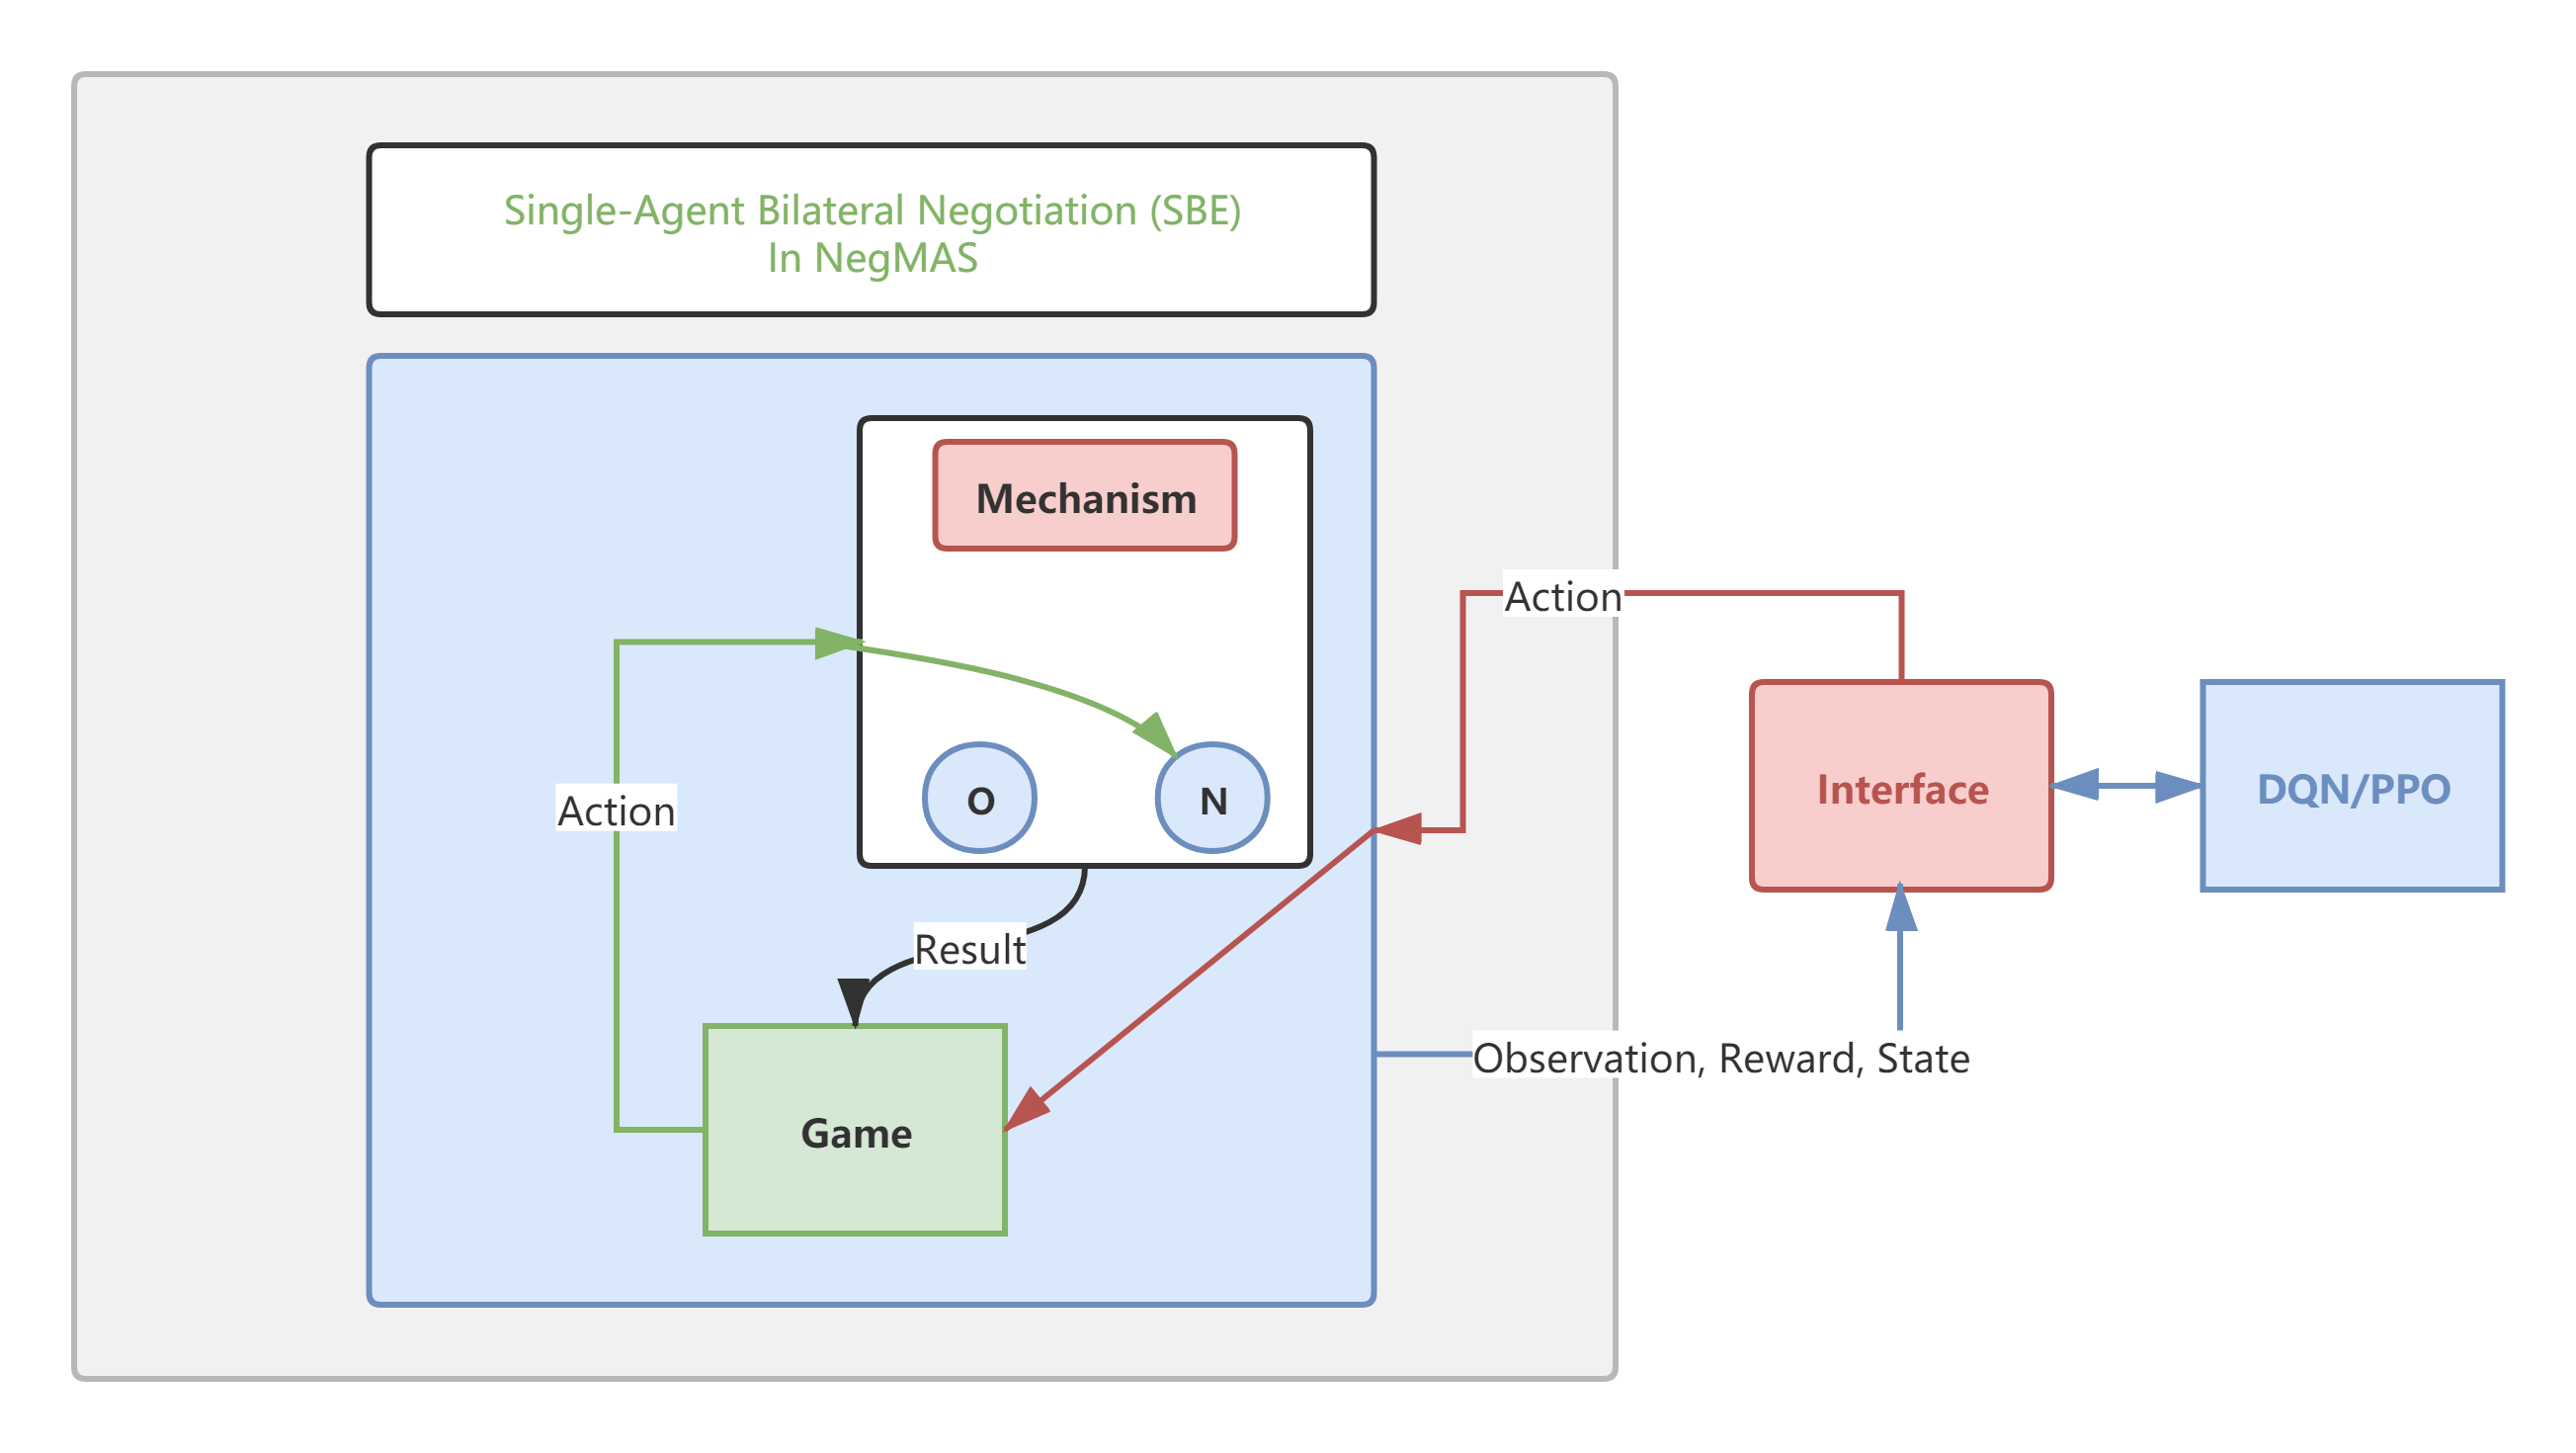
\includegraphics[width=0.80\textwidth]{./images/sbe.png}
\caption{Model for single agent bilateral negotiation based on NegMAS}
\label{fig:environment-single-agent}
\end{figure}

\subsection{Single-Agent Environment} \label{single-agent-env}
The interface of the OpenAI Gym Environments is designed for one agent as standard. Nevertheless, it must be examined how the \gls{sbe} can be represented via this interface and controlled by the controller. The methods of the interface for the \gls{sbe} are therefore defined below. 

\paragraph{STEP} Firstly, sets up but not performs the action received from \gls{rl} algorithms for the negotiator. Then, run the negotiation mechanism (such as \gls{saom} ) for one step. All actions will be perfomed by the negotiation mechanism. Finally, the function returns four parameters.

\begin{itemize}
	\item Observation: Offer proposed by opponent and current relative time.
	\item Reward: Utility value of the current offer and extra reward when an agreement is reached.
	\item Done: Reach the final state or there is no agreement within the maximum running time.
	\item Info: State of the negotiation mechanism, extra info used for evaluation.
\end{itemize}

\paragraph{RESET} Resets the environment to an initial state and returns an initial observation, initial observation contains negotiators' intial observation and other information relative to the definition of observation space. Reset the time and current step. Create a new negotiation mechanism session.
\paragraph{RENDER} This application is not required because there is no visual output.
\paragraph{CLOSE}  This application is not needed because there is no need to save the data created by the environment.
\paragraph{SEED} Sets the seed for this env's random number generator(s), such as negotiation mechanism.

\subsection{Game} \label{game}
In addition to implementing the official \gls{openai gym} \texttt{Env} interface, class \texttt{Game} is designed to control the entire negotiation mechanism. The purpose of this design is to reduce the modification of negotiatioin mechanism of \gls{negmas}. In this class, there are some parameters, which are received from the mechanism of \gls{negmas} and passed to the \gls{rl} algorithms as additional information. The two main methods are defined below.
 
\paragraph{STEP} Checks the state of \texttt{Game}, runs the negotiation mechanism for one step.
\paragraph{STEP\_FORWARD} Sets the key logic for the running of the negotiation mechanism, because negotiator can learn different strategy in \gls{sbe}. 

\subsection{Challenges of the environment}
\gls{openai gym} provides an unified interface for custome environment. But it has some problems, which cannot be directly solved by the interface. These problems occurred during environmental design and will be listed and discussed in the following sections. 

\subsubsection{Design of Action Space and Observation Space}
One relevant consideration is related to \gls{rl} In \parencite{Bakker2019RLBOAAM}, the author study a modular \gls{rl} based on BOA (Bidding strategy, Opponent model and Acceptance condition) framwork which is an extension of the work done in \parencite{Bakker2019RLBOAAM}. This framework of \gls{rlboa} implements an agent that uses tabular Q-learning to learn the bidding strategy by discretizing the continuous state/action space (not an optimal solution for large state/action spaces as it may lead to curse of dimensionality and cause the loss of relevant information about the state/action domain structure too) \parencite{bagga2020deep}. 
Compared with tabular Q-learning, deep reinforcement learning algorithms use neural networks to solve this problem.
 
There are two possible approaches to implementing deep reinforcement learning for this learning case:

The first method: The output size of neural network is directly related to the size of the action space, in other words, it is related to the size of negotiation issues. 

The second method: Discrete action space replaced by continuous action space. Before apply the action, filter invalid actions and scale valid actions.

\subsubsection{Design of Reward Function}
The reward function is the focus of the implementation of the \gls{rl} algorithm. It is easy to understand, \gls{rl} learns startegies by evaluating the value of actions. Therefore, it is very necessary to design a good reward function. In \gls{sbe}, the utility function defined by \texttt{Negotiator} can be used as a calculation tool to get the current offer reward, which can be intuitively set as part of the reward function.  

\subsection{Analysis of the reinforcement learning algorithms}
\subsubsection{Policy Optimization vs. Q-Learning}
PPO vs. DQN

\subsection{Conclusion}


\section{\gls{scml} with \gls{openai gym}}
\subsection{Configuration}
\subsubsection{Negotiation Issues}
\paragraph{Standard \gls{scml}} Negotiation issues are multi-issues, Quantity, Time and Price. 
\paragraph{\gls{scml-oneshot}} Negotiation issues are multi-issues, Quantity and Price. Time is not important in this simulation world. All contracts will be executed at the same step in which agents reach agreements.

\subsection{Model}
The model consists of six parts, environment \texttt{\gls{mcbe}}, Scenario, World, Agent, Interface and \gls{madrl} algorithms.
All six parts are needed to be rewritten according to \gls{scml} and \gls{openai gym}. 

Entire model is shown in \ref{fig:environment-multi-agent}
\begin{figure}[htbp]
\centering
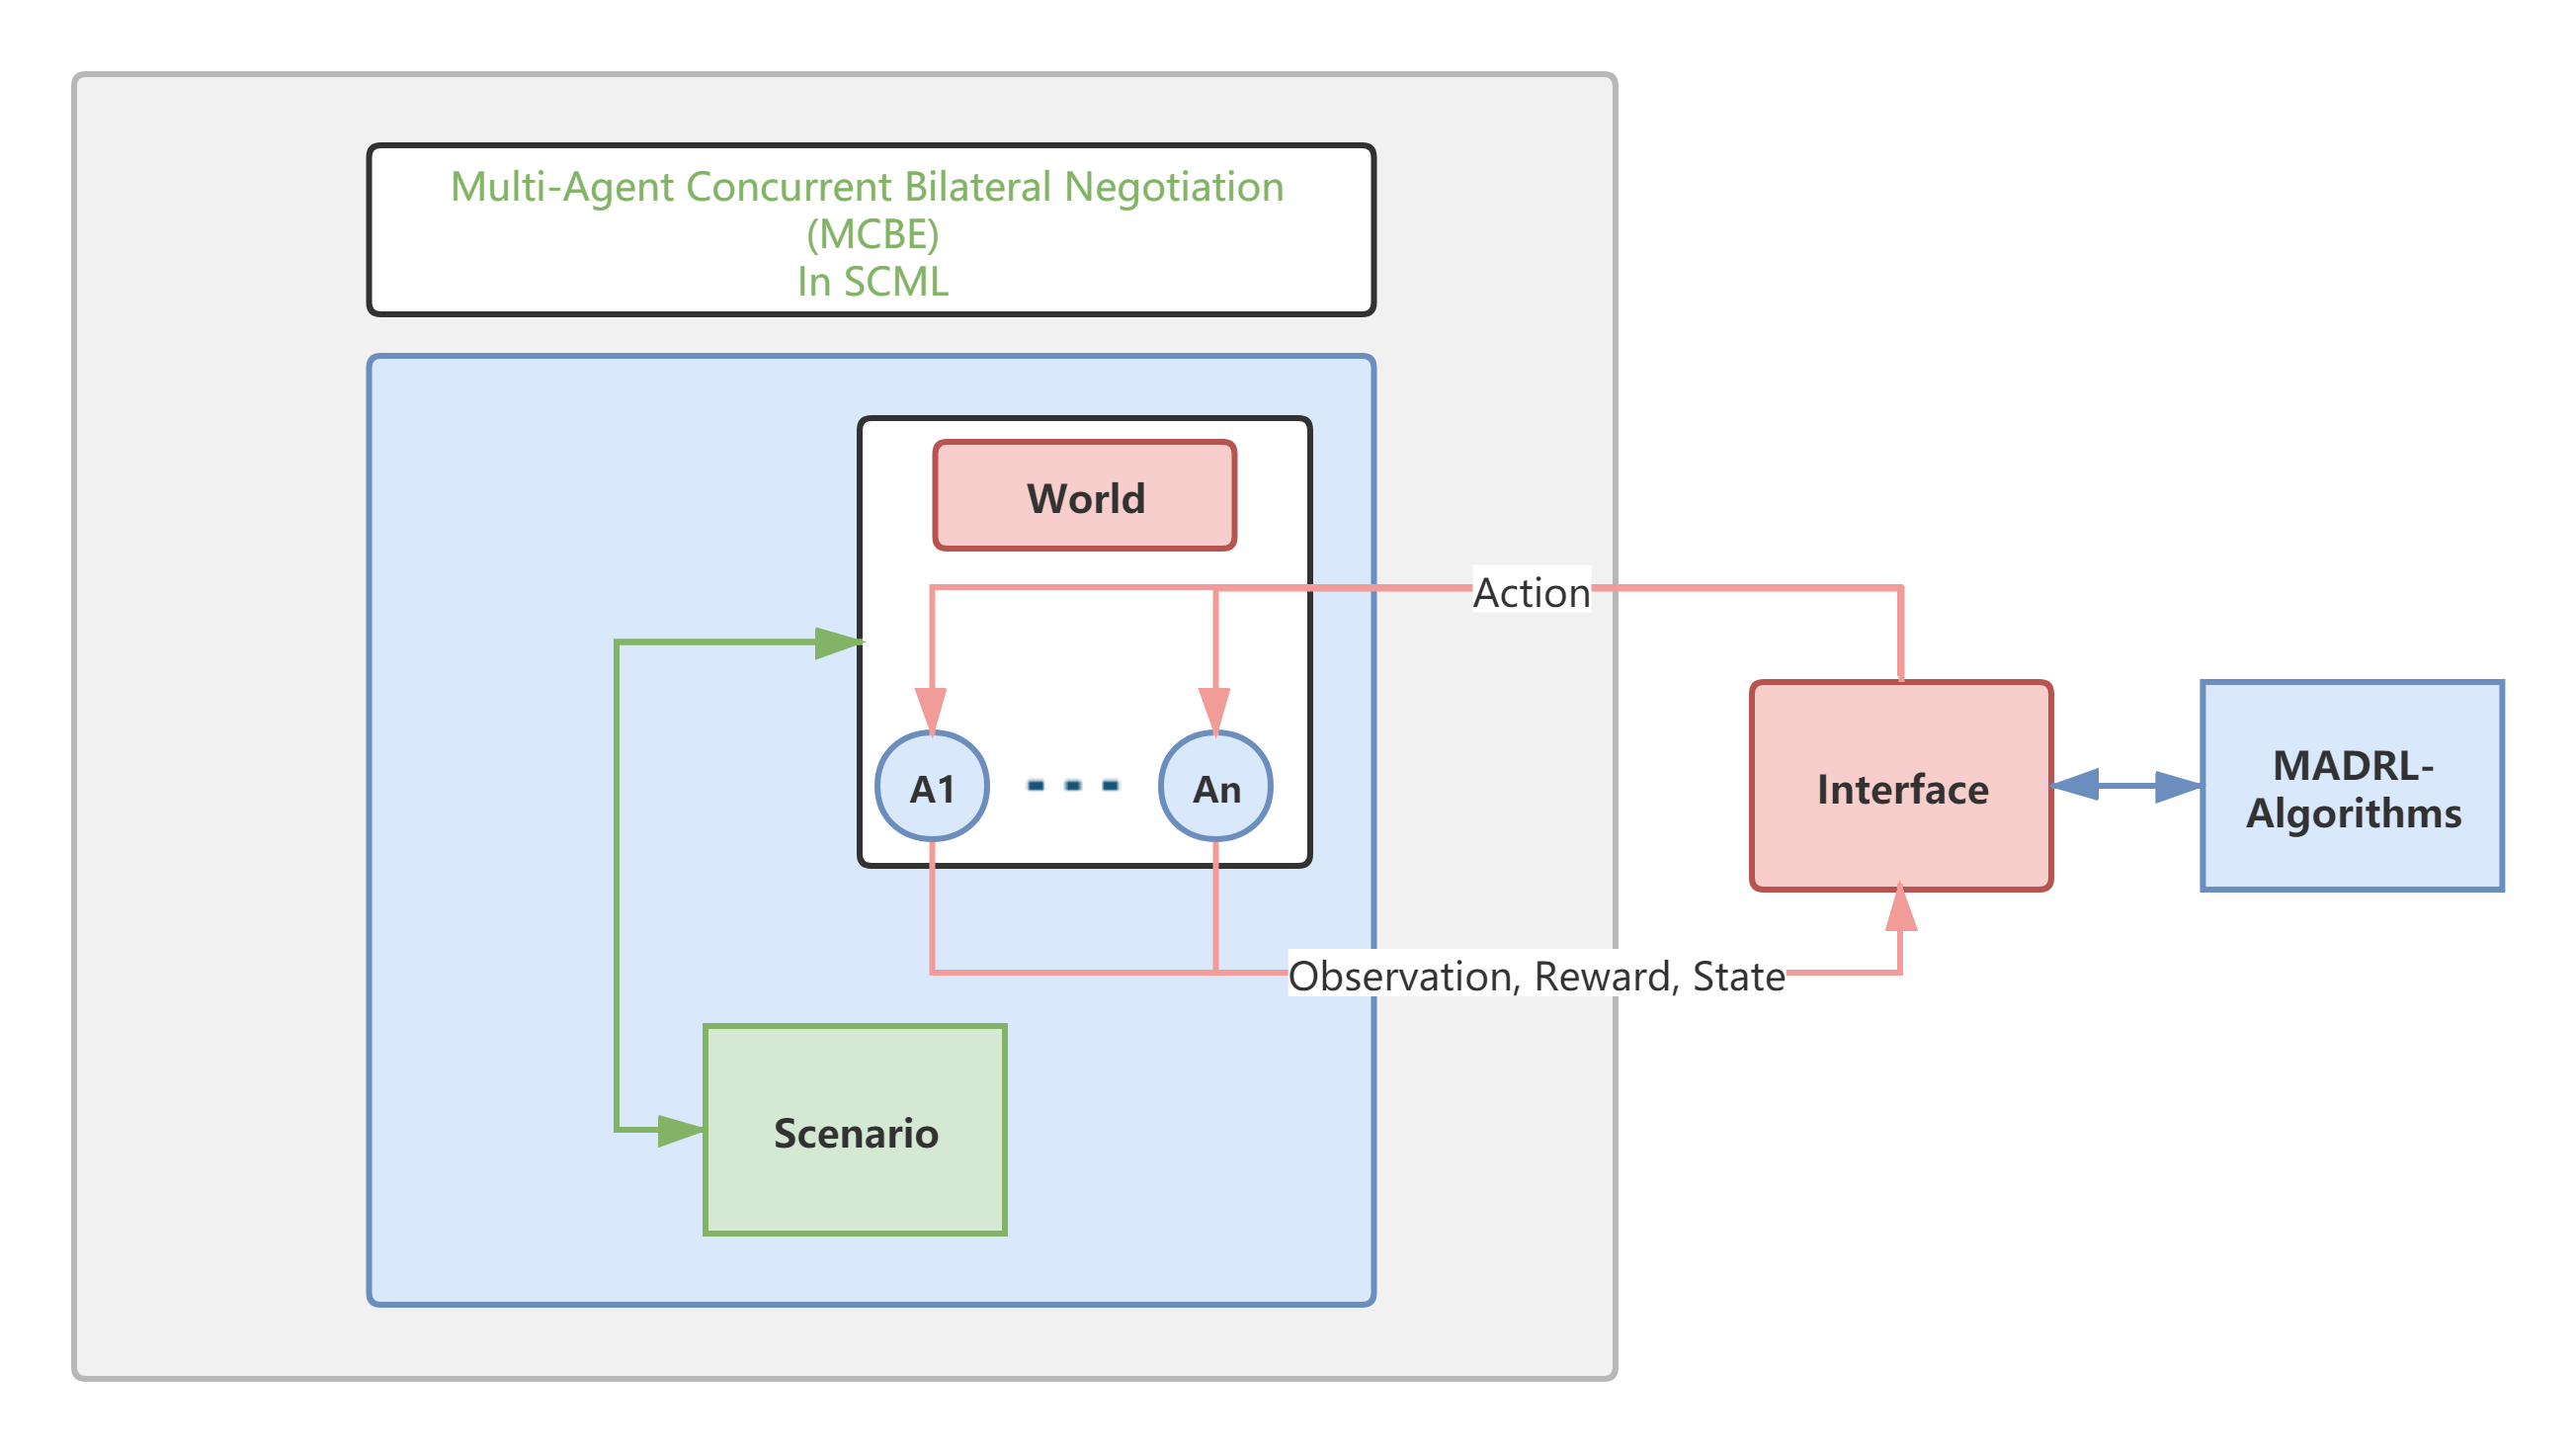
\includegraphics[width=0.9\textwidth]{./images/MCBE.png}
\caption{Model for Multi-Agent Concurrent Bilateral Negotiation based on \gls{scml}}
\label{fig:environment-multi-agent}
\end{figure}

\subsection{Multi-Agent Environment} \label{multi-agent-env}
In order to be able to realize deep reinforcement learning for multi-agent with an OpenAI Gym Environment, the interface would have to be expanded. In the following, alternative possibilities for using an OpenAI Gym Environment for \gls{marl} are discussed. 
Since \gls{mcbe} realizes \gls{openai gym} \texttt{env} interface methods, a new method named \texttt{run} is added to execute entire episode.

\paragraph{STEP} Runs the simulated world for one step. Not important in this case. 
\paragraph{RESET} Resets the environment(MCBE) and other related parameters to an initial state after every episode and returns an initial observation.
\paragraph{RENDER} This application is not required because there is no visual output.
\paragraph{CLOSE} This application is not needed because there is no need to save the data created by
the environment.
\paragraph{SEED} Sets the seed for this env’s random number generator(s)
\paragraph{RUN} Runs entire episode. After a negotiation step, the rewards, observations, actions, etc. are stored in the memory buffer. 
\begin{itemize}
	\item Observation: Current offer in negotiation mechanism. The observations of all agents are combined in one list. Agent can only access to its local observation during decentralised execution.
	\item Reward: Sum reward of all learnable agents. Reward of single agent is the sum of utility value of the current offer after one negotiation step and profit of agent after one simulation step.
	\item Done: Reaches the final state (last step of simulation world) or the maximum running time.
	\item State: State of environment. It can be replaced by \texttt{Observation}.
\end{itemize}

\subsection{Scenario} \label{scenario}
Scenario describes the structure of simulation world. It is similar as the assisted method \texttt{Game} in \gls{sbe} and provides logic for generating and resetting the world. With the help of Scenario, many scenarios can be created without changing of \gls{mcbe}. Figure \ref{fig:supply-chain-scenario-1} diagrams a simple scenario.

\begin{figure}[htbp]
\centering
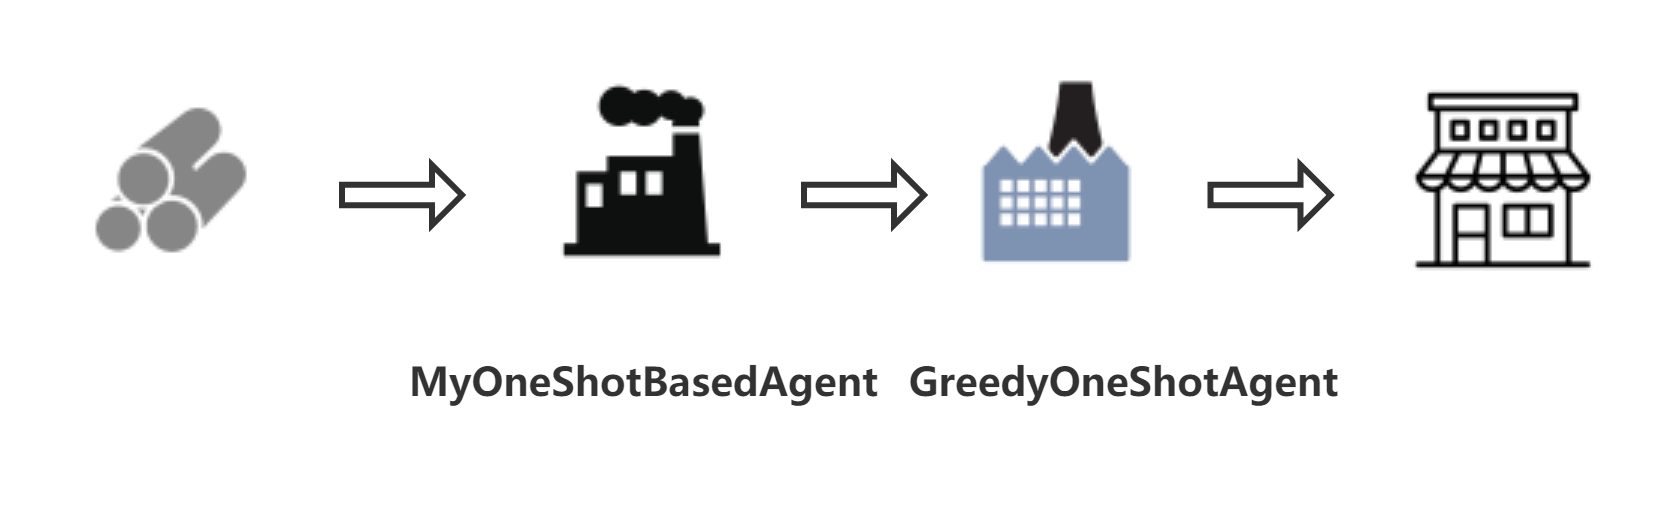
\includegraphics[width=0.9\textwidth]{./images/supply-chain-scenario-1.png}
\caption{Example of supply chain scenario, \gls{my-one-shot-drl-agent} vs. \gls{greedy-one-shot-agent}}
\label{fig:supply-chain-scenario-1}
\end{figure}

Scenario Interface consists three normal functions and four callback functions passed to \gls{mcbe}.

\paragraph{MAKE\_WORLD} Creates instance of game or training world.
\paragraph{RESET\_WORLD} Sets the world to the initial state.
\paragraph{RESET\_AGENT} Resets agent, returns initial observation.
\paragraph{CALLBACK} OBSERVATION, REWARD, DONE and INFO

\subsection{Challenges of the environment}
\subsubsection{Combination with \gls{scml}}
Compared with \gls{sbe}, \gls{mcbe} can not directly call the function designed in official \gls{scml}. \texttt{Step} in \gls{scml-oneshot} is one simulation step. In one simulation step, many negotiation steps will be performed. The action of the agent is a \texttt{proposal}, so it needs to be meticulous to control every step of the negotiation mechanism in the simulation world. The class \texttt{TrainWorld} inherited from SCMLOneShotWorld achieves this goal.
\subsubsection{Design of Reward Function} 
In \gls{scm} world, the goal of the agent is to maximize profit at the end of the simulation. It is difficult to train an agent based on the reward signal alone. With the concept of reward shape \ref{related-work:sparse-reward} the reward signal can be splited as two parts: utility of agent after every simulated step and profit at the end of simulation. The utility function of agent is defined in the equation \ref{equation:utility-agent}.

\begin{equation} \label{equation:utility-agent}
\begin{aligned}
u_{f}\left(C^{i}, C^{o}\right)=&-\sum_{c \in C^{i}}\left(p_{c} q_{c}\right)+\sum_{c \in \bar{C}^{o}}\left(p_{c} q_{c}\right)-\\
                               &\sum_{c \in C^{i}}\left(p_{c} q_{c}\right)-m_{f} P_{f}-\gamma_{f} \operatorname{tp}\left(p_{f}^{i}, d\right) Q_{f}^{o>i}-\alpha_{f} \operatorname{tp}\left(p_{f}^{o}, d\right) Q_{f}^{i>0}
\end{aligned}
\end{equation}
Where $C^{i}$ denotes the set of input contracts plus the exogenous input contracts. $C^{o}$ denotes the set of output contracts plus the exogenous output contracts. Price and quantity of the contract $c$ are formed by $p_c$ and $q_c$, respectively. Because the agent can only sell what it can produce, the set of satisfiable output contracts can be defined as $\bar{C}^{o}$. $Q^{o>i}$ is simply the quantity to be bought according to $C^{i}$ but is never sold.

\subsection{Analysis of the reinforcement learning algorithms}
\subsubsection{Independent Learning vs. Centralized Learning}
\paragraph{Non-stationary environment}
Traditional reinforcement learning approaches such as Q-Learning or policy gradient
are poorly suited to multi-agent environments. One issue is that each agent’s policy is changing as training progresses, and the environment becomes non-stationary from the perspective of any individual agent (in a way that is not explainable by changes in the agent’s own policy).

\subsubsection{\gls{maddpg} vs. \gls{qmix}}
Centralised learning of joint actions can naturally handle coordination problems and avoids non-stationarity, but is hard to scale, as the joint action space grows exponentially in the number of agents. In \parencite{Rashid2018}, author proposed a neural network to transform the centralised state into the weights of another neural network. This second neural network is constrained to be monotonic with respect to its inputs by keeping its weights positive. This feature makes it possible to learn when there are many agents.

\subsection{Conclusion}
